\documentclass[11pt]{article}
\usepackage[margin=1in]{geometry}
\usepackage{amsmath,amssymb,booktabs,graphicx,caption,hyperref,xcolor,enumitem,float}
\usepackage[T1]{fontenc}
\usepackage{lmodern}
\usepackage[round]{natbib}
\hypersetup{colorlinks=true,linkcolor=blue!50!black,citecolor=blue!50!black,urlcolor=blue!50!black}
\captionsetup{font=small,labelfont=bf}
\setlist{itemsep=2pt,topsep=4pt}
\newcommand{\rs}{r^{*}}

\title{Financial Conditions, $r^*$, and the Transmission of Monetary Policy Surprises}
\author{Draft for discussion}
\date{1 November 2026}

\begin{document}
\maketitle

\begin{abstract}
\noindent High-frequency monetary policy surprises identify policy shocks cleanly, but their estimated effects on unemployment and inflation in post-1994 data are often weak or puzzling. We show that two features of the monetary transmission mechanism resolve much of this. First, policy reaches the economy through financial conditions as a whole---long-term yields, equity valuations and the dollar---not through a single short-term rate. Second, the level of interest rates must be measured relative to the neutral rate $\rs$, which trended down for most of the period. We propagate surprises measured in 30-minute FOMC windows through a mixed-frequency model in which daily financial variables drive monthly unemployment and core inflation. With a nominal two-year yield as the only channel, the familiar puzzles appear: unemployment falls and industrial production rises after a tightening. Adding a market-based financial conditions index turns the responses conventional; measuring rates and the index relative to the Laubach--Williams $\rs$ makes them precise and stable. A policy move that raises the two-year yield by 1 percentage point raises the unemployment gap by about 0.3 percentage point within a year and lowers the core price level by about 0.5 percent after two years---similar to, and for unemployment larger and more persistent than, the best recent estimates \citep{bauer2023}. The two ingredients complement existing remedies based on information effects and on purging predictable surprises.
\end{abstract}

\section{Introduction}
The high-frequency identification of monetary policy shocks is one of the major empirical advances in macroeconomics. Changes in interest-rate futures and Treasury yields in narrow windows around FOMC announcements isolate news about policy from other news \citep{kuttner2001,gurkaynak2005}, and their effects on asset prices are estimated precisely \citep{bernanke2005,nakamura2018}. Using these surprises to learn about the effects of policy on output, unemployment and inflation has been harder. In samples that start in the 1990s, the estimated responses are often small, imprecise or of the wrong sign \citep{ramey2016}. The literature has offered two main explanations and remedies. One is that policy announcements reveal the Federal Reserve's information about the economy, so that a surprise tightening also signals good news \citep{romer2000,nakamura2018,jarocinski2020,miranda2021}. The other is that surprises are partly predictable from public data that predate the announcement, reflecting the market's misperception of the Fed's response to the economy; orthogonalizing them restores conventional and larger responses \citep{bauer2023,bauer2023aer}. A third strand stresses that the transmission of policy through financial markets must be modeled: \citet{gertler2015} use the one-year yield and the excess bond premium, and \citet{caldara2019} show that omitting credit spreads, to which policy reacts, attenuates all responses.

This note proposes a simpler and complementary explanation, rooted in the transmission mechanism itself. Policy affects spending through the whole configuration of financial conditions---the cost of long-term credit, the value of wealth, and the exchange rate \citep{boivin2010}---and what matters for spending is the level of real interest rates relative to their neutral level $\rs$, which fell substantially from the 1990s to the 2010s \citep{laubach2003,holston2017,kiley2020}. Empirical models that carry a high-frequency surprise forward through a single nominal short-term rate neglect both features. The first omission matters because the surprise moves long yields, equities and the dollar along with the short rate, and these components carry much of the effect on activity. The second matters because, over the post-1994 period, rates trended down with $\rs$ while activity trended up; a reduced-form link between the level of rates and activity then partly reflects these opposing trends rather than the cyclical stance of policy.

We take a direct route. The shock is the \citet{nakamura2018} policy-news surprise, measured in 30-minute windows (253 FOMC announcements, 1994--2026). Its impact on the two-year yield and, when included, on a market-based financial conditions index (FCI) is read off the window, where macroeconomic variables do not move. A daily model carries the financial variables forward from the announcement day, and monthly unemployment and core inflation respond to monthly averages of the daily variables, as in a standard monthly VAR. The model respects the timing of each announcement within its month, which addresses the temporal-aggregation problem stressed by \citet{kilian2024} and \citet{chudik2022}. The FCI is the market index of a companion note \citep{fcinote}: its weights on the 10-year yield, equity valuation and the real dollar are their responses to the same policy news, and it is built in three steps---nominal, real, and relative to $\rs$.

The evidence builds in four steps. With the nominal two-year yield as the only channel, the post-1994 puzzles appear: unemployment falls after a tightening, significantly with richer lag structures, prices do not move, and industrial production rises. Adding the FCI turns the unemployment response conventional. Measuring rates in real terms changes little. Measuring rates and the FCI relative to $\rs$ is decisive: the unemployment response becomes significant at horizons of one to three years for every lag length, the core price level falls significantly, and industrial production falls. Neither ingredient works alone: removing $\rs$ without the FCI leaves the puzzle in place, and the FCI without $\rs$ gives the right sign but imprecise estimates. The magnitudes are close to the benchmark of \citet{bauer2023}: unemployment rises about 0.3 percentage point in the first year against their 0.2, and stays higher for longer; the price level falls by about 0.5 percent after two years, as in their estimates. We obtain these results from FOMC announcements alone, without orthogonalizing the surprises.

These results complement rather than compete with the information-effect and predictability literatures. Our propagation is estimated from the reduced-form link between financial conditions and the economy, so it is less exposed to the correlation between surprises and prior news that biases proxy VARs \citep{bauer2023}, and the surprise reaches macro variables only through financial conditions, which screens out information channels that bypass markets. Both mechanisms may therefore be at work alongside ours. Our point is that two standard features of the transmission mechanism---financial conditions as a whole, and the level of rates relative to $\rs$---go a long way toward resolving the puzzles on their own, and that they have been absent from the high-frequency-identification literature.\footnote{This statement is based on the papers we have read, including those cited above; we have not found high-frequency studies that propagate the shock through a broad financial conditions index or measure the policy rate relative to $\rs$. The closest is \citet{caldara2019}, who add a credit spread.}

\section{Data and method}
\textbf{Surprises and window responses.} The shock is the Nakamura--Steinsson policy-news factor from the San Francisco Fed's U.S.\ Monetary Policy Event-Study Database \citep{acosta2025}: the first principal component of 30-minute changes in five short-term interest-rate futures around 253 FOMC announcements, February 1994 to September 2026. We scale it so that the two-year Treasury yield rises 1 percentage point in the window. The window response of the FCI (0.99 per percentage point) is computed from the 30-minute changes in the 10-year yield, the S\&P 500 and the dollar index in the same database, combined with the FCI's weights. Unemployment and prices are zero in the window.

\textbf{Financial conditions.} The FCI is the market index of \citet{fcinote}: a weighted sum of the 10-year Treasury yield, equity valuation (cyclically adjusted price--earnings ratio, CAPE) and the real broad dollar, with weights equal to their responses to the same policy news, so that a unit of the index is the effect of a policy move that raises the two-year yield 1 percentage point. It comes in three versions, built in the same steps as in that note. \emph{Nominal}: the variables as measured. \emph{Real}: the 10-year yield net of 10-year expected inflation. \emph{$\rs$-gap} (baseline): the real 10-year yield net of the one-sided Laubach--Williams $\rs$ (New York Fed, current estimates), and equities as the gap between the earnings yield and $\rs$. The two-year yield follows the same rule: nominal; net of two-year expected inflation \citep[Cleveland Fed;][]{haubrich2012}; and net of expected inflation and $\rs$. Daily versions follow the daily 10-year yield, CAPE and dollar and are shifted, smoothly within each month, so that their monthly averages equal the monthly indexes exactly; the adjustments for expected inflation and $\rs$ move slowly, so the window responses are the same in every version.

\textbf{Model.} The model has a daily and a monthly block. In the daily block, the two-year yield and (when included) the FCI follow a heterogeneous autoregression in their 1-, 5-, 22- and 66-day averages and respond to the current and previous month's unemployment gap and core inflation (estimated 1990--2026). In the monthly block, the unemployment gap (the CBO-based gap of the companion note) and core PCE inflation are rows of a monthly VAR with $L$ lags of each and $L$ lags of the monthly averages of the daily financial variables, estimated by OLS over February 1994--September 2026 with March--December 2020 excluded; $L$ is 3, 6 or 12. Within each month macro conditions are set first, and markets respond to them; in the announcement month, macro variables have not yet moved. The response to a surprise is computed by placing the window impact on the announcement day (drawn from the empirical distribution of FOMC dates within the month), simulating the daily block forward, averaging within months, and iterating the monthly block. This is a restricted mixed-frequency VAR in the sense of \citet{ghysels2016}, with equal weights within the month; the restriction is the one implied by a standard monthly VAR, and we could not reject it for unemployment.

\textbf{Identifying assumption.} The surprise affects unemployment and prices only through the variables in the daily block, and the economy responds to a given change in those variables in the same way whatever caused it. The first part is weaker the more complete the set of financial variables; the second is the assumption behind any use of financial conditions indexes to summarize the stance of policy \citep{hatzius2010,ajello2023}. A direct regression of unemployment on the surprises that does not impose it \citep{chudik2022,chudik2026} is about ten times less precise and cannot discriminate between our estimates and zero.

\textbf{Inference.} We resample announcements (which re-estimates the window impact and the distribution of announcement dates) and residuals of the monthly equations, 200 draws. We report 68 and 90 percent intervals. Recent high-frequency studies report 90 percent bands \citep{bauer2023,caldara2019,miranda2021,ramey2016}, \citet{gertler2015} 95 percent, and \citet{jarocinski2020} both 68 and 90 percent.

\section{Results}
Table~\ref{tab:u} and Table~\ref{tab:p} report the responses of the unemployment gap and the core PCE price level at 12, 24 and 36 months, for 3, 6 and 12 monthly lags, at each step. Figure~\ref{fig:steps} shows the four key cases.

\begin{table}[H]\centering\small
\caption{Unemployment gap (percentage points), per 1 percentage point policy-induced rise in the two-year yield}\label{tab:u}
{\setlength{\tabcolsep}{4pt}\begin{tabular}{llccccccccc}
\toprule
 & & \multicolumn{3}{c}{12 months} & \multicolumn{3}{c}{24 months} & \multicolumn{3}{c}{36 months}\\
\cmidrule(lr){3-5}\cmidrule(lr){6-8}\cmidrule(lr){9-11}
Rate & FCI & 3 & 6 & 12 & 3 & 6 & 12 & 3 & 6 & 12 \\
\midrule
Nominal & no & 0.07 & $-$0.13 & $-$0.27$^{**}$ & 0.36$^{\dagger}$ & 0.10 & $-$0.19 & 0.53$^{**}$ & 0.29 & $-$0.00 \\
Nominal & yes & 0.44$^{**}$ & 0.36$^{**}$ & 0.28$^{**}$ & 0.76$^{**}$ & 0.75$^{**}$ & 0.63$^{**}$ & 0.76$^{**}$ & 0.83$^{**}$ & 0.77$^{**}$ \\
\midrule
Real & no & 0.14$^{\dagger}$ & $-$0.04 & $-$0.20$^{**}$ & 0.33$^{**}$ & 0.12 & $-$0.13 & 0.42$^{**}$ & 0.23 & $-$0.01 \\
Real & yes & 0.44$^{**}$ & 0.38$^{**}$ & 0.29$^{**}$ & 0.65$^{**}$ & 0.65$^{**}$ & 0.59$^{**}$ & 0.57$^{**}$ & 0.64$^{**}$ & 0.64$^{**}$ \\
\midrule
$r^*$-gap & no & 0.19$^{**}$ & 0.10 & $-$0.03 & 0.34$^{**}$ & 0.21 & 0.04 & 0.38$^{**}$ & 0.25$^{\dagger}$ & 0.07 \\
$r^*$-gap & yes & 0.40$^{**}$ & 0.37$^{**}$ & 0.36$^{**}$ & 0.47$^{**}$ & 0.48$^{**}$ & 0.50$^{**}$ & 0.35$^{**}$ & 0.40$^{**}$ & 0.43$^{**}$ \\
\bottomrule
\end{tabular}
}
\par\smallskip\begin{minipage}{0.95\textwidth}\footnotesize Columns: horizon and number of monthly lags. $^{**}$: 90 percent interval excludes zero; $^{*}$: 68 percent interval excludes zero. Rates and FCI at each step as described in Section~2. \citet{bauer2023}, benchmark: $+0.19$ at 12 months (90 percent band excludes zero), $+0.17$ and $+0.15$ at 24 and 36 months (band includes zero), read from their Figure~8.\end{minipage}
\end{table}

\begin{table}[H]\centering\small
\caption{Core PCE price level (percent), per 1 percentage point policy-induced rise in the two-year yield}\label{tab:p}
{\setlength{\tabcolsep}{4pt}\begin{tabular}{llccccccccc}
\toprule
 & & \multicolumn{3}{c}{12 months} & \multicolumn{3}{c}{24 months} & \multicolumn{3}{c}{36 months}\\
\cmidrule(lr){3-5}\cmidrule(lr){6-8}\cmidrule(lr){9-11}
Rate & FCI & 3 & 6 & 12 & 3 & 6 & 12 & 3 & 6 & 12 \\
\midrule
Nominal & no & 0.01 & 0.06 & 0.01 & $-$0.08 & 0.03 & 0.05 & $-$0.17 & $-$0.07 & 0.03 \\
Nominal & yes & $-$0.09 & $-$0.07 & $-$0.10 & $-$0.28$^{\dagger}$ & $-$0.24$^{\dagger}$ & $-$0.23 & $-$0.42$^{\dagger}$ & $-$0.41$^{\dagger}$ & $-$0.36$^{\dagger}$ \\
\midrule
Real & no & $-$0.10$^{\dagger}$ & $-$0.02 & $-$0.07 & $-$0.19$^{\dagger}$ & $-$0.08 & $-$0.06 & $-$0.26$^{\dagger}$ & $-$0.16 & $-$0.08 \\
Real & yes & $-$0.17$^{\dagger}$ & $-$0.14$^{\dagger}$ & $-$0.18$^{**}$ & $-$0.33$^{\dagger}$ & $-$0.32$^{\dagger}$ & $-$0.31$^{\dagger}$ & $-$0.44$^{\dagger}$ & $-$0.47$^{**}$ & $-$0.41$^{\dagger}$ \\
\midrule
$r^*$-gap & no & $-$0.15$^{\dagger}$ & $-$0.13$^{\dagger}$ & $-$0.19$^{**}$ & $-$0.22$^{\dagger}$ & $-$0.26$^{\dagger}$ & $-$0.31$^{\dagger}$ & $-$0.28$^{\dagger}$ & $-$0.39 & $-$0.44$^{\dagger}$ \\
$r^*$-gap & yes & $-$0.18$^{\dagger}$ & $-$0.25$^{**}$ & $-$0.33$^{**}$ & $-$0.28$^{\dagger}$ & $-$0.48$^{**}$ & $-$0.61$^{**}$ & $-$0.37$^{\dagger}$ & $-$0.68$^{**}$ & $-$0.84$^{**}$ \\
\bottomrule
\end{tabular}
}
\par\smallskip\begin{minipage}{0.95\textwidth}\footnotesize See Table~\ref{tab:u}. \citet{bauer2023}, benchmark (CPI): $-0.36$, $-0.48$ and $-0.6$ at 12, 24 and 36 months, 90 percent bands exclude zero.\end{minipage}
\end{table}

\begin{figure}[H]\centering
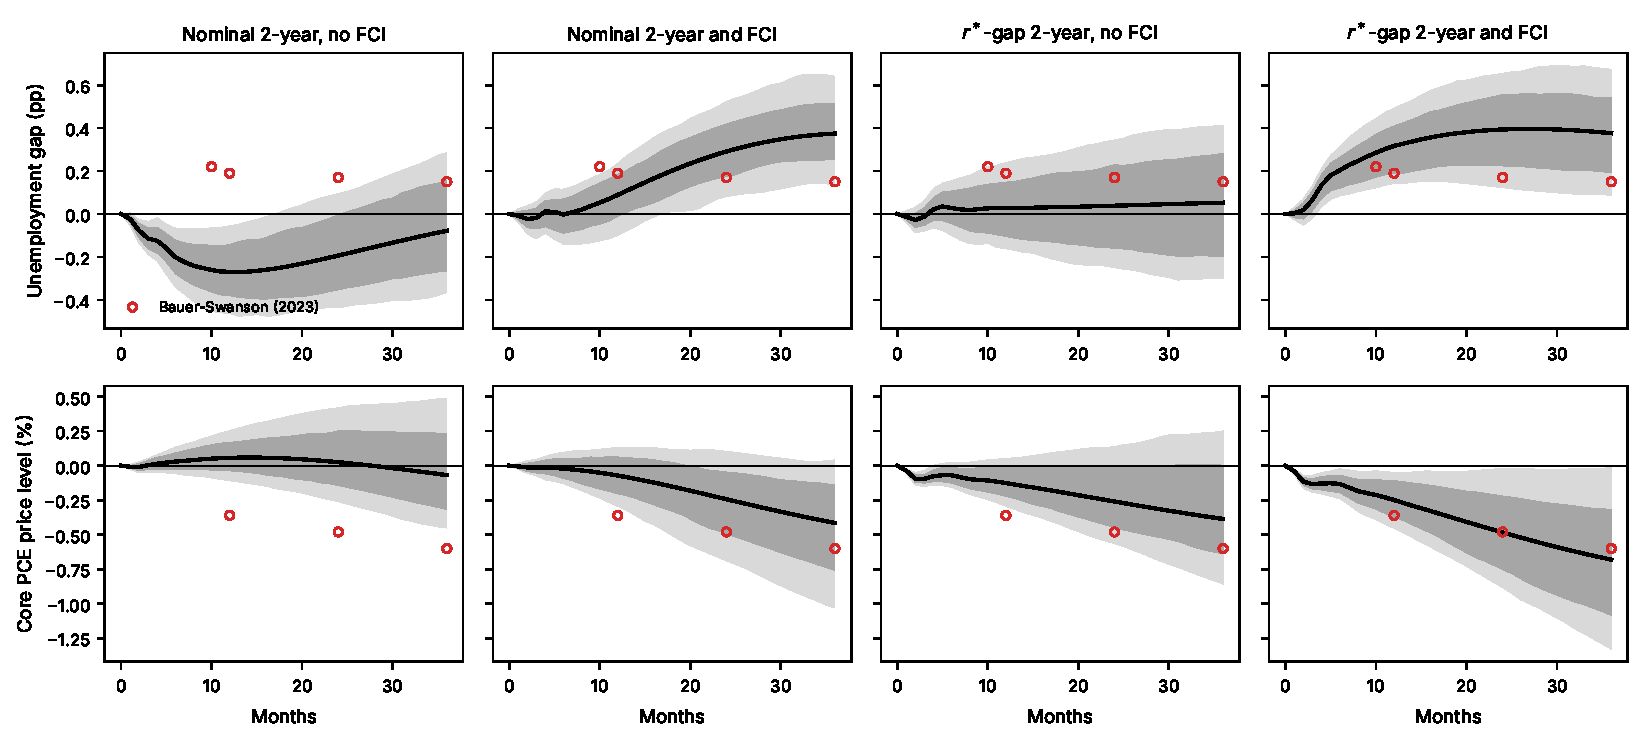
\includegraphics[width=\textwidth]{figures/fig1_steps.pdf}
\caption{Responses to a policy move that raises the two-year yield 1 percentage point (6 lags). Dark band: 68 percent; light band: 90 percent. Circles: \citet{bauer2023}, read from their Figure~8.}\label{fig:steps}
\end{figure}

\textbf{Step 1: the standard set-up reproduces the puzzles.} With the nominal two-year yield as the only channel---the policy indicator of \citet{bauer2023}---unemployment falls after a tightening, significantly with 6 and 12 lags, and the price level does not move. This is the post-1994 pattern documented by \citet{ramey2016} and the one \citet{bauer2023} obtain with unadjusted surprises.

\textbf{Step 2: financial conditions.} Adding the FCI turns the unemployment response conventional at every horizon and lag length. It is significant at 36 months, but at 12 months it is weak with 6 and 12 lags, and the price level falls without being significant at conventional levels. STEP2_68

\textbf{Step 3: real rates.} Measuring the two-year yield and the FCI net of expected inflation changes little, as in the companion note, where the nominal and real indexes are close after 1990: expected inflation moved little in this period.

\textbf{Step 4: rates relative to $\rs$.} Measuring the two-year yield and the FCI relative to $\rs$ is decisive, but only together. Without the FCI, the $\rs$-gap rate leaves unemployment insignificant. With it, unemployment rises by 0.30--0.34 percentage point at 12 months and 0.34--0.38 at 36 months, significant at the 90 percent level at every horizon and lag length and nearly identical across lag lengths. The price level falls by 0.48--0.61 percent at 24 months with 6 and 12 lags, significant at the 90 percent level. STEP4_68

\textbf{Comparison with \citet{bauer2023}.} Their benchmark proxy VAR (1973--2020, with surprises from FOMC announcements and Chair speeches, orthogonalized to pre-announcement news) gives a peak unemployment response of about 0.2 percentage point after 10 months and a CPI decline of about 0.5 percent after two years, per percentage point on the two-year yield. Our step-4 estimates match the price response and give a larger and more persistent unemployment response, with intervals that exclude zero through 36 months where theirs include zero after about a year and a half. Their estimates use 30 years of instrument data, Chair speeches and orthogonalization; ours use FOMC windows alone and no orthogonalization.

\section{Robustness}
\textbf{Industrial production.} Adding industrial production to the monthly block (Table~\ref{tab:ip}) leaves the pattern for unemployment and prices unchanged. Without the FCI, industrial production rises after a tightening at every step; with the FCI it falls; at the $\rs$ step it falls about 0.9 percent at 12 months, significantly with 6 and 12 lags, against about 1.5 percent in \citet{bauer2023}, and recovers faster.

\begin{table}[H]\centering\small
\caption{Industrial production (percent), monthly block with industrial production added}\label{tab:ip}
{\setlength{\tabcolsep}{4pt}\begin{tabular}{llccccccccc}
\toprule
 & & \multicolumn{3}{c}{12 months} & \multicolumn{3}{c}{24 months} & \multicolumn{3}{c}{36 months}\\
\cmidrule(lr){3-5}\cmidrule(lr){6-8}\cmidrule(lr){9-11}
Rate & FCI & 3 & 6 & 12 & 3 & 6 & 12 & 3 & 6 & 12 \\
\midrule
Nominal & no & 1.06$^{**}$ & 1.26$^{**}$ & 1.65$^{**}$ & 1.03$^{\dagger}$ & 1.26$^{\dagger}$ & 1.64$^{**}$ & 1.16$^{\dagger}$ & 1.00$^{\dagger}$ & 1.10$^{\dagger}$ \\
Nominal & yes & $-$0.16 & $-$0.29 & 0.11 & $-$0.09 & $-$0.04 & 0.15 & 0.45 & 0.39 & 0.43 \\
\midrule
Real & no & 0.64$^{\dagger}$ & 0.77$^{**}$ & 1.13$^{**}$ & 0.72 & 0.97$^{\dagger}$ & 1.28$^{**}$ & 0.87$^{\dagger}$ & 0.85$^{\dagger}$ & 0.91$^{\dagger}$ \\
Real & yes & $-$0.33 & $-$0.52 & $-$0.23 & $-$0.11 & $-$0.11 & $-$0.01 & 0.42 & 0.31 & 0.34 \\
\midrule
$r^*$-gap & no & 0.13 & $-$0.04 & 0.27 & 0.13 & 0.23 & 0.32 & 0.31 & 0.44 & 0.21 \\
$r^*$-gap & yes & $-$0.84$^{**}$ & $-$1.05$^{**}$ & $-$0.95$^{**}$ & $-$0.46$^{\dagger}$ & $-$0.48 & $-$0.80$^{**}$ & 0.18 & 0.08 & $-$0.21 \\
\bottomrule
\end{tabular}
}
\par\smallskip\begin{minipage}{0.95\textwidth}\footnotesize See Table~\ref{tab:u}. \citet{bauer2023}: about $-1.5$, $-1.0$ and $-0.85$ at 12, 24 and 36 months, read from their Figure~8.\end{minipage}
\end{table}

\textbf{Which trend?} Table~\ref{tab:rob} replaces the Laubach--Williams estimate with \citet{kiley2020}'s, and replaces the real and $\rs$ adjustments with two statistical trends: a quadratic time trend in every monthly equation, and the two-year yield measured relative to its trailing 8-year average. ROB_TEXT

\begin{table}[H]\centering\small
\caption{Alternative trends: unemployment gap (top) and core PCE price level (bottom)}\label{tab:rob}
{\setlength{\tabcolsep}{3pt}\begin{tabular}{llccccccccc}
\toprule
 & & \multicolumn{3}{c}{12 months} & \multicolumn{3}{c}{24 months} & \multicolumn{3}{c}{36 months}\\
\cmidrule(lr){3-5}\cmidrule(lr){6-8}\cmidrule(lr){9-11}
Rate & FCI & 3 & 6 & 12 & 3 & 6 & 12 & 3 & 6 & 12 \\
\midrule
$r^*$-gap, Laubach--Williams (baseline) & none & 0.08 & 0.03 & $-$0.08 & 0.16$^{\dagger}$ & 0.04 & $-$0.15$^{\dagger}$ & 0.20$^{\dagger}$ & 0.05 & $-$0.16 \\
$r^*$-gap, Laubach--Williams (baseline) & $r^*$-gap (LW) & 0.30$^{**}$ & 0.32$^{**}$ & 0.34$^{**}$ & 0.38$^{**}$ & 0.39$^{**}$ & 0.41$^{**}$ & 0.34$^{**}$ & 0.38$^{**}$ & 0.37$^{**}$ \\
\midrule
2-year $-$ 9--10y forward rate & none & $-$0.23$^{**}$ & $-$0.22$^{**}$ & $-$0.26$^{**}$ & $-$0.33$^{**}$ & $-$0.24$^{\dagger}$ & $-$0.35$^{**}$ & $-$0.34$^{**}$ & $-$0.22$^{\dagger}$ & $-$0.30$^{\dagger}$ \\
2-year $-$ 9--10y forward rate & forward-gap & $-$0.20$^{\dagger}$ & $-$0.10 & $-$0.08 & $-$0.39$^{**}$ & $-$0.15 & $-$0.22 & $-$0.44$^{**}$ & $-$0.18 & $-$0.29 \\
\midrule
$r^*$-gap, Kiley & none & 0.00 & $-$0.11 & $-$0.22$^{**}$ & 0.06 & $-$0.10 & $-$0.29$^{**}$ & 0.09 & $-$0.07 & $-$0.25$^{\dagger}$ \\
$r^*$-gap, Kiley & $r^*$-gap (Kiley) & 0.38$^{**}$ & 0.28$^{**}$ & 0.15$^{\dagger}$ & 0.47$^{**}$ & 0.36$^{\dagger}$ & 0.14 & 0.37$^{**}$ & 0.30$^{\dagger}$ & 0.09 \\
\midrule
Nominal + quadratic trend & none & 0.07 & $-$0.13 & $-$0.27$^{**}$ & 0.36$^{\dagger}$ & 0.10 & $-$0.19 & 0.53$^{**}$ & 0.29 & $-$0.00 \\
Nominal + quadratic trend & nominal & 0.44$^{**}$ & 0.36$^{**}$ & 0.28$^{**}$ & 0.76$^{**}$ & 0.75$^{**}$ & 0.63$^{**}$ & 0.76$^{**}$ & 0.83$^{**}$ & 0.77$^{**}$ \\
Nominal + quadratic trend & real & 0.41$^{**}$ & 0.32$^{**}$ & 0.25$^{\dagger}$ & 0.69$^{**}$ & 0.67$^{**}$ & 0.57$^{**}$ & 0.68$^{**}$ & 0.74$^{**}$ & 0.70$^{**}$ \\
\midrule
2-year $-$ 8-year average & none & $-$0.22$^{**}$ & $-$0.30$^{**}$ & $-$0.36$^{**}$ & $-$0.23$^{\dagger}$ & $-$0.28$^{\dagger}$ & $-$0.46$^{**}$ & $-$0.22 & $-$0.21 & $-$0.40$^{**}$ \\
2-year $-$ 8-year average & nominal & 0.23$^{**}$ & 0.18$^{\dagger}$ & 0.15$^{\dagger}$ & 0.38$^{**}$ & 0.36$^{**}$ & 0.27$^{\dagger}$ & 0.34$^{**}$ & 0.36$^{**}$ & 0.27$^{**}$ \\
2-year $-$ 8-year average & real & 0.25$^{**}$ & 0.19$^{**}$ & 0.15$^{\dagger}$ & 0.37$^{**}$ & 0.36$^{**}$ & 0.28$^{\dagger}$ & 0.31$^{**}$ & 0.34$^{**}$ & 0.29$^{\dagger}$ \\
2-year $-$ 8-year average & $r^*$-gap (LW) & 0.06 & 0.08 & 0.14$^{\dagger}$ & 0.10$^{\dagger}$ & 0.15$^{\dagger}$ & 0.18$^{\dagger}$ & 0.08 & 0.15$^{\dagger}$ & 0.18 \\
\bottomrule
\end{tabular}
}\par\medskip
{\setlength{\tabcolsep}{3pt}\begin{tabular}{llccccccccc}
\toprule
 & & \multicolumn{3}{c}{12 months} & \multicolumn{3}{c}{24 months} & \multicolumn{3}{c}{36 months}\\
\cmidrule(lr){3-5}\cmidrule(lr){6-8}\cmidrule(lr){9-11}
Rate & FCI & 3 & 6 & 12 & 3 & 6 & 12 & 3 & 6 & 12 \\
\midrule
2-year $r^*$-gap, Laubach--Williams (baseline) & none & $-$0.27$^{**}$ & $-$0.22$^{**}$ & $-$0.23$^{**}$ & $-$0.45$^{**}$ & $-$0.51$^{**}$ & $-$0.52$^{**}$ & $-$0.55$^{**}$ & $-$0.70$^{**}$ & $-$0.80$^{**}$ \\
2-year $r^*$-gap, Laubach--Williams (baseline) & nominal & $-$0.25$^{**}$ & $-$0.28$^{**}$ & $-$0.30$^{**}$ & $-$0.42$^{**}$ & $-$0.59$^{**}$ & $-$0.66$^{**}$ & $-$0.50$^{**}$ & $-$0.75$^{**}$ & $-$0.92$^{**}$ \\
2-year $r^*$-gap, Laubach--Williams (baseline) & real & $-$0.26$^{**}$ & $-$0.29$^{**}$ & $-$0.33$^{**}$ & $-$0.44$^{**}$ & $-$0.59$^{**}$ & $-$0.70$^{**}$ & $-$0.52$^{**}$ & $-$0.75$^{**}$ & $-$0.97$^{**}$ \\
2-year $r^*$-gap, Laubach--Williams (baseline) & $r^*$-gap & $-$0.34$^{**}$ & $-$0.33$^{**}$ & $-$0.33$^{**}$ & $-$0.53$^{**}$ & $-$0.68$^{**}$ & $-$0.72$^{**}$ & $-$0.57$^{**}$ & $-$0.85$^{**}$ & $-$0.97$^{**}$ \\
\midrule
2-year $r^*$-gap, Kiley & none & $-$0.23$^{**}$ & $-$0.16$^{\dagger}$ & $-$0.18$^{**}$ & $-$0.37$^{**}$ & $-$0.34$^{\dagger}$ & $-$0.29$^{\dagger}$ & $-$0.44$^{**}$ & $-$0.48$^{\dagger}$ & $-$0.41$^{\dagger}$ \\
2-year $r^*$-gap, Kiley & nominal & $-$0.23$^{**}$ & $-$0.24$^{**}$ & $-$0.21$^{\dagger}$ & $-$0.39$^{**}$ & $-$0.50$^{**}$ & $-$0.41$^{\dagger}$ & $-$0.43$^{**}$ & $-$0.61$^{**}$ & $-$0.53$^{\dagger}$ \\
2-year $r^*$-gap, Kiley & real & $-$0.25$^{**}$ & $-$0.25$^{**}$ & $-$0.25$^{**}$ & $-$0.40$^{**}$ & $-$0.51$^{**}$ & $-$0.46$^{\dagger}$ & $-$0.44$^{**}$ & $-$0.62$^{**}$ & $-$0.58$^{\dagger}$ \\
2-year $r^*$-gap, Kiley & $r^*$-gap & $-$0.34$^{**}$ & $-$0.33$^{**}$ & $-$0.29$^{**}$ & $-$0.48$^{**}$ & $-$0.62$^{**}$ & $-$0.58$^{**}$ & $-$0.47$^{**}$ & $-$0.69$^{**}$ & $-$0.68$^{**}$ \\
\midrule
2-year $-$ 9--10y forward rate & none & 0.01 & $-$0.04 & $-$0.08 & 0.04 & $-$0.04 & $-$0.06 & 0.05 & $-$0.06 & $-$0.07 \\
2-year $-$ 9--10y forward rate & nominal & $-$0.05 & $-$0.12 & $-$0.14$^{\dagger}$ & $-$0.07 & $-$0.21 & $-$0.25 & $-$0.06 & $-$0.22 & $-$0.31 \\
2-year $-$ 9--10y forward rate & real & $-$0.06 & $-$0.14$^{\dagger}$ & $-$0.18$^{\dagger}$ & $-$0.07 & $-$0.21 & $-$0.30$^{\dagger}$ & $-$0.06 & $-$0.21 & $-$0.37 \\
2-year $-$ 9--10y forward rate & $r^*$-gap & $-$0.22$^{**}$ & $-$0.27$^{**}$ & $-$0.30$^{**}$ & $-$0.29$^{**}$ & $-$0.48$^{**}$ & $-$0.62$^{**}$ & $-$0.30$^{\dagger}$ & $-$0.53$^{**}$ & $-$0.81$^{**}$ \\
\midrule
2-year $-$ 8-year average & none & $-$0.08 & $-$0.06 & $-$0.08 & $-$0.25$^{\dagger}$ & $-$0.27$^{\dagger}$ & $-$0.23$^{\dagger}$ & $-$0.37$^{\dagger}$ & $-$0.47$^{\dagger}$ & $-$0.45$^{\dagger}$ \\
2-year $-$ 8-year average & nominal & $-$0.13$^{\dagger}$ & $-$0.15$^{\dagger}$ & $-$0.16$^{\dagger}$ & $-$0.27$^{\dagger}$ & $-$0.38$^{**}$ & $-$0.39$^{\dagger}$ & $-$0.31$^{\dagger}$ & $-$0.49$^{**}$ & $-$0.56$^{\dagger}$ \\
2-year $-$ 8-year average & real & $-$0.14$^{\dagger}$ & $-$0.15$^{\dagger}$ & $-$0.18$^{\dagger}$ & $-$0.28$^{\dagger}$ & $-$0.37$^{**}$ & $-$0.42$^{\dagger}$ & $-$0.32$^{\dagger}$ & $-$0.49$^{**}$ & $-$0.61$^{\dagger}$ \\
2-year $-$ 8-year average & $r^*$-gap & $-$0.25$^{**}$ & $-$0.24$^{**}$ & $-$0.24$^{**}$ & $-$0.46$^{**}$ & $-$0.61$^{**}$ & $-$0.63$^{**}$ & $-$0.56$^{**}$ & $-$0.83$^{**}$ & $-$0.96$^{**}$ \\
\bottomrule
\end{tabular}
}
\par\smallskip\begin{minipage}{0.95\textwidth}\footnotesize See Table~\ref{tab:u}. FCI column: the FCI version used (no FCI; nominal; real; $\rs$-gap). The 8-year average and Laubach--Williams trends (two-year expected inflation plus $\rs$) are close until 2015 (averages 5.3 and 5.5 percent over 1994--2007; 2.3 and 2.5 over 2008--2015) and diverge after 2016 (1.4 and 3.6).\end{minipage}
\end{table}

\section{Conclusion}
CONCLUSION

\begin{thebibliography}{99}\small
\bibitem[Acosta et al.(2025)]{acosta2025} Acosta, M., A. Ajello, M. Bauer, F. Loria and S. Miranda-Agrippino (2025), ``Financial Market Effects of FOMC Communication: Evidence from a New Event-Study Database,'' Federal Reserve Bank of San Francisco Working Paper 2025-30.
\bibitem[Ajello et al.(2023)]{ajello2023} Ajello, A., M. Cavallo, G. Favara, W. Peterman, J. Schindler and N. Sinha (2023), ``A New Index to Measure U.S. Financial Conditions,'' FEDS Notes, Board of Governors of the Federal Reserve System, June 30.
\bibitem[Bauer and Swanson(2023a)]{bauer2023} Bauer, M. D. and E. T. Swanson (2023a), ``A Reassessment of Monetary Policy Surprises and High-Frequency Identification,'' NBER Macroeconomics Annual 37, 87--155.
\bibitem[Bauer and Swanson(2023b)]{bauer2023aer} Bauer, M. D. and E. T. Swanson (2023b), ``An Alternative Explanation for the `Fed Information Effect','' American Economic Review 113(3), 664--700.
\bibitem[Bernanke and Kuttner(2005)]{bernanke2005} Bernanke, B. S. and K. N. Kuttner (2005), ``What Explains the Stock Market's Reaction to Federal Reserve Policy?'' Journal of Finance 60(3), 1221--1257.
\bibitem[Boivin et al.(2010)]{boivin2010} Boivin, J., M. T. Kiley and F. S. Mishkin (2010), ``How Has the Monetary Transmission Mechanism Evolved Over Time?'' in B. M. Friedman and M. Woodford (eds.), Handbook of Monetary Economics, Vol.\ 3A, 369--422.
\bibitem[Caldara and Herbst(2019)]{caldara2019} Caldara, D. and E. Herbst (2019), ``Monetary Policy, Real Activity, and Credit Spreads: Evidence from Bayesian Proxy SVARs,'' American Economic Journal: Macroeconomics 11(1), 157--192.
\bibitem[Chudik and Georgiadis(2022)]{chudik2022} Chudik, A. and G. Georgiadis (2022), ``Estimation of Impulse Response Functions When Shocks Are Observed at a Higher Frequency Than Outcome Variables,'' Journal of Business and Economic Statistics 40(3), 965--979.
\bibitem[Chudik and Kilian(2026)]{chudik2026} Chudik, A. and L. Kilian (2026), ``Mean Group and Pooled Mixed-Frequency Estimators of Responses of Low-Frequency Variables to High-Frequency Shocks,'' Federal Reserve Bank of Dallas Working Paper 2603.
\bibitem[FCI note(2026)]{fcinote} Companion note (2026), ``A Simple Market-Based Financial Conditions Index: Weights from Policy News, Dynamics from a Transparent VAR, Measured Relative to $r^*$,'' draft.
\bibitem[Gertler and Karadi(2015)]{gertler2015} Gertler, M. and P. Karadi (2015), ``Monetary Policy Surprises, Credit Costs, and Economic Activity,'' American Economic Journal: Macroeconomics 7(1), 44--76.
\bibitem[Ghysels(2016)]{ghysels2016} Ghysels, E. (2016), ``Macroeconomics and the Reality of Mixed Frequency Data,'' Journal of Econometrics 193(2), 294--314.
\bibitem[G\"urkaynak et al.(2005)]{gurkaynak2005} G\"urkaynak, R. S., B. Sack and E. T. Swanson (2005), ``Do Actions Speak Louder Than Words? The Response of Asset Prices to Monetary Policy Actions and Statements,'' International Journal of Central Banking 1(1), 55--93.
\bibitem[Hatzius et al.(2010)]{hatzius2010} Hatzius, J., P. Hooper, F. Mishkin, K. Schoenholtz and M. Watson (2010), ``Financial Conditions Indexes: A Fresh Look after the Financial Crisis,'' NBER Working Paper 16150.
\bibitem[Haubrich et al.(2012)]{haubrich2012} Haubrich, J., G. Pennacchi and P. Ritchken (2012), ``Inflation Expectations, Real Rates, and Risk Premia: Evidence from Inflation Swaps,'' Review of Financial Studies 25(5), 1588--1629.
\bibitem[Holston et al.(2017)]{holston2017} Holston, K., T. Laubach and J. C. Williams (2017), ``Measuring the Natural Rate of Interest: International Trends and Determinants,'' Journal of International Economics 108, S59--S75.
\bibitem[Jaroci\'nski and Karadi(2020)]{jarocinski2020} Jaroci\'nski, M. and P. Karadi (2020), ``Deconstructing Monetary Policy Surprises---The Role of Information Shocks,'' American Economic Journal: Macroeconomics 12(2), 1--43.
\bibitem[Kiley(2020)]{kiley2020} Kiley, M. T. (2020), ``What Can the Data Tell Us about the Equilibrium Real Interest Rate?'' International Journal of Central Banking 16(3), 181--209.
\bibitem[Kilian(2024)]{kilian2024} Kilian, L. (2024), ``How to Construct Monthly VAR Proxies Based on Daily Surprises in Futures Markets,'' Journal of Economic Dynamics and Control 168, 104966.
\bibitem[Kuttner(2001)]{kuttner2001} Kuttner, K. N. (2001), ``Monetary Policy Surprises and Interest Rates: Evidence from the Fed Funds Futures Market,'' Journal of Monetary Economics 47(3), 523--544.
\bibitem[Laubach and Williams(2003)]{laubach2003} Laubach, T. and J. C. Williams (2003), ``Measuring the Natural Rate of Interest,'' Review of Economics and Statistics 85(4), 1063--1070.
\bibitem[Miranda-Agrippino and Ricco(2021)]{miranda2021} Miranda-Agrippino, S. and G. Ricco (2021), ``The Transmission of Monetary Policy Shocks,'' American Economic Journal: Macroeconomics 13(3), 74--107.
\bibitem[Nakamura and Steinsson(2018)]{nakamura2018} Nakamura, E. and J. Steinsson (2018), ``High-Frequency Identification of Monetary Non-Neutrality: The Information Effect,'' Quarterly Journal of Economics 133(3), 1283--1330.
\bibitem[Ramey(2016)]{ramey2016} Ramey, V. A. (2016), ``Macroeconomic Shocks and Their Propagation,'' in J. B. Taylor and H. Uhlig (eds.), Handbook of Macroeconomics, Vol.\ 2A, 71--162.
\bibitem[Romer and Romer(2000)]{romer2000} Romer, C. D. and D. H. Romer (2000), ``Federal Reserve Information and the Behavior of Interest Rates,'' American Economic Review 90(3), 429--457.
\end{thebibliography}
\end{document}
